\documentclass[12pt, twoside]{article}
\usepackage[francais]{babel}
\usepackage[T1]{fontenc}
\usepackage[latin1]{inputenc}
\usepackage[left=7mm, right=7mm, top=7mm, bottom=7mm]{geometry}
\usepackage{float}
\usepackage{graphicx}
\usepackage{array}
\usepackage{multirow}
\usepackage{amsmath,amssymb,mathrsfs} 
\usepackage{soul}
\usepackage{textcomp}
\usepackage{eurosym}
\usepackage{lscape} 
 \usepackage{variations}
\usepackage{tabvar}
 
\pagestyle{empty} 

\title{\ul{\textbf{A propos des droites}}}
\date{} 

\begin{document}
\maketitle


\section{Vocabulaire et notation}

\begin{center}
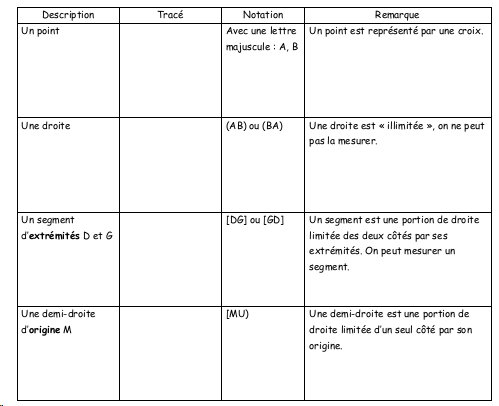
\includegraphics[width=12cm]{images/tableau.jpg}
\end{center}



 
\medskip


\ul{D�finition}: Des \textbf{points align�s} sont des points  qui appartiennent
� une m�me droite.

\enskip

\ul{Exemples}:

\begin{tabular}{cc}
\begin{minipage}{9cm}

\begin{center}
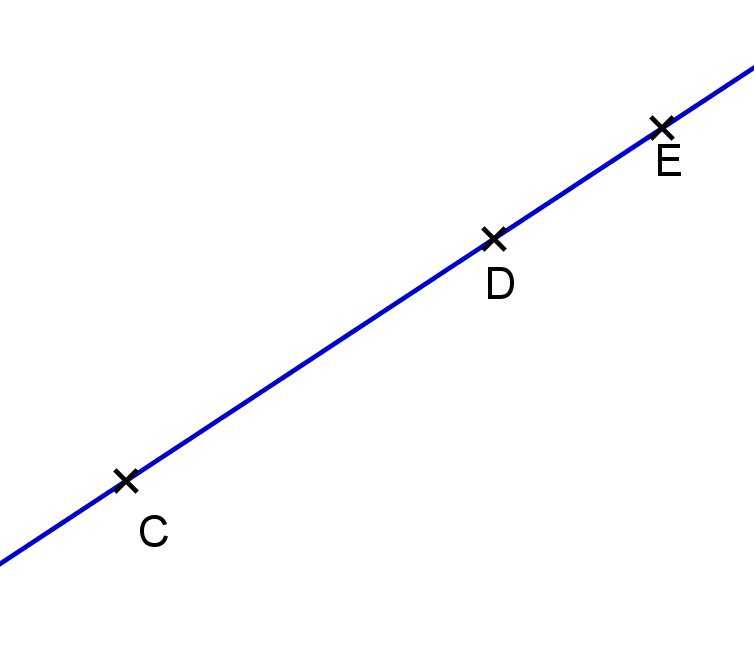
\includegraphics[width=4cm]{images/CDE.png}
\end{center}


Les points C, D et E sont align�s. Le point C 

appartient � la droite (DE). 

On note: $C \in (DE)$.
\end{minipage}
& 
\begin{minipage}{9cm}

\begin{center}
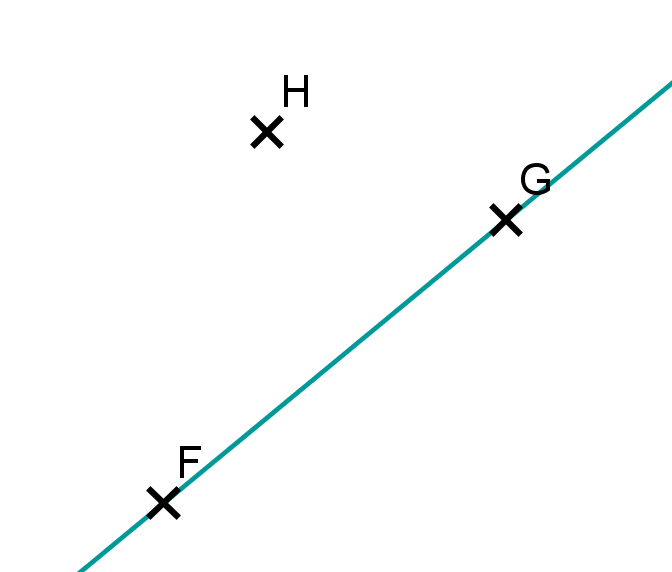
\includegraphics[width=4cm]{images/FGH.png}
\end{center}

Les points F,G et H ne sont pas align�s. Le point H n'appartient pas � la
droite (FG).

ON note: $H \notin  (FG)$.
\end{minipage}
\end{tabular}







\section{Droites s�cantes, droites perpendiculaires et droites parall�les}


\subsection{D�finitions}

\ul{D�finition}: Deux droites \textbf{s�cantes} sont deux droites qui ont un
seul point commun.




\begin{tabular}{cc}
\begin{minipage}{12cm}



A est le seul point commun aux droites ($d_1$) et ($d_2$). On dit que:


$\bullet$ ($d_1$) et ($d_2$) sont \textbf{s�cantes en A}.

$\bullet$ ($d_1$) et ($d_2$) se \textbf{coupent en A}.


$\bullet$ A est le \textbf{point d'intersection} des droites ($d_1$) et ($d_2$).


 
\end{minipage}
& 
\begin{minipage}{6cm}

\begin{center}
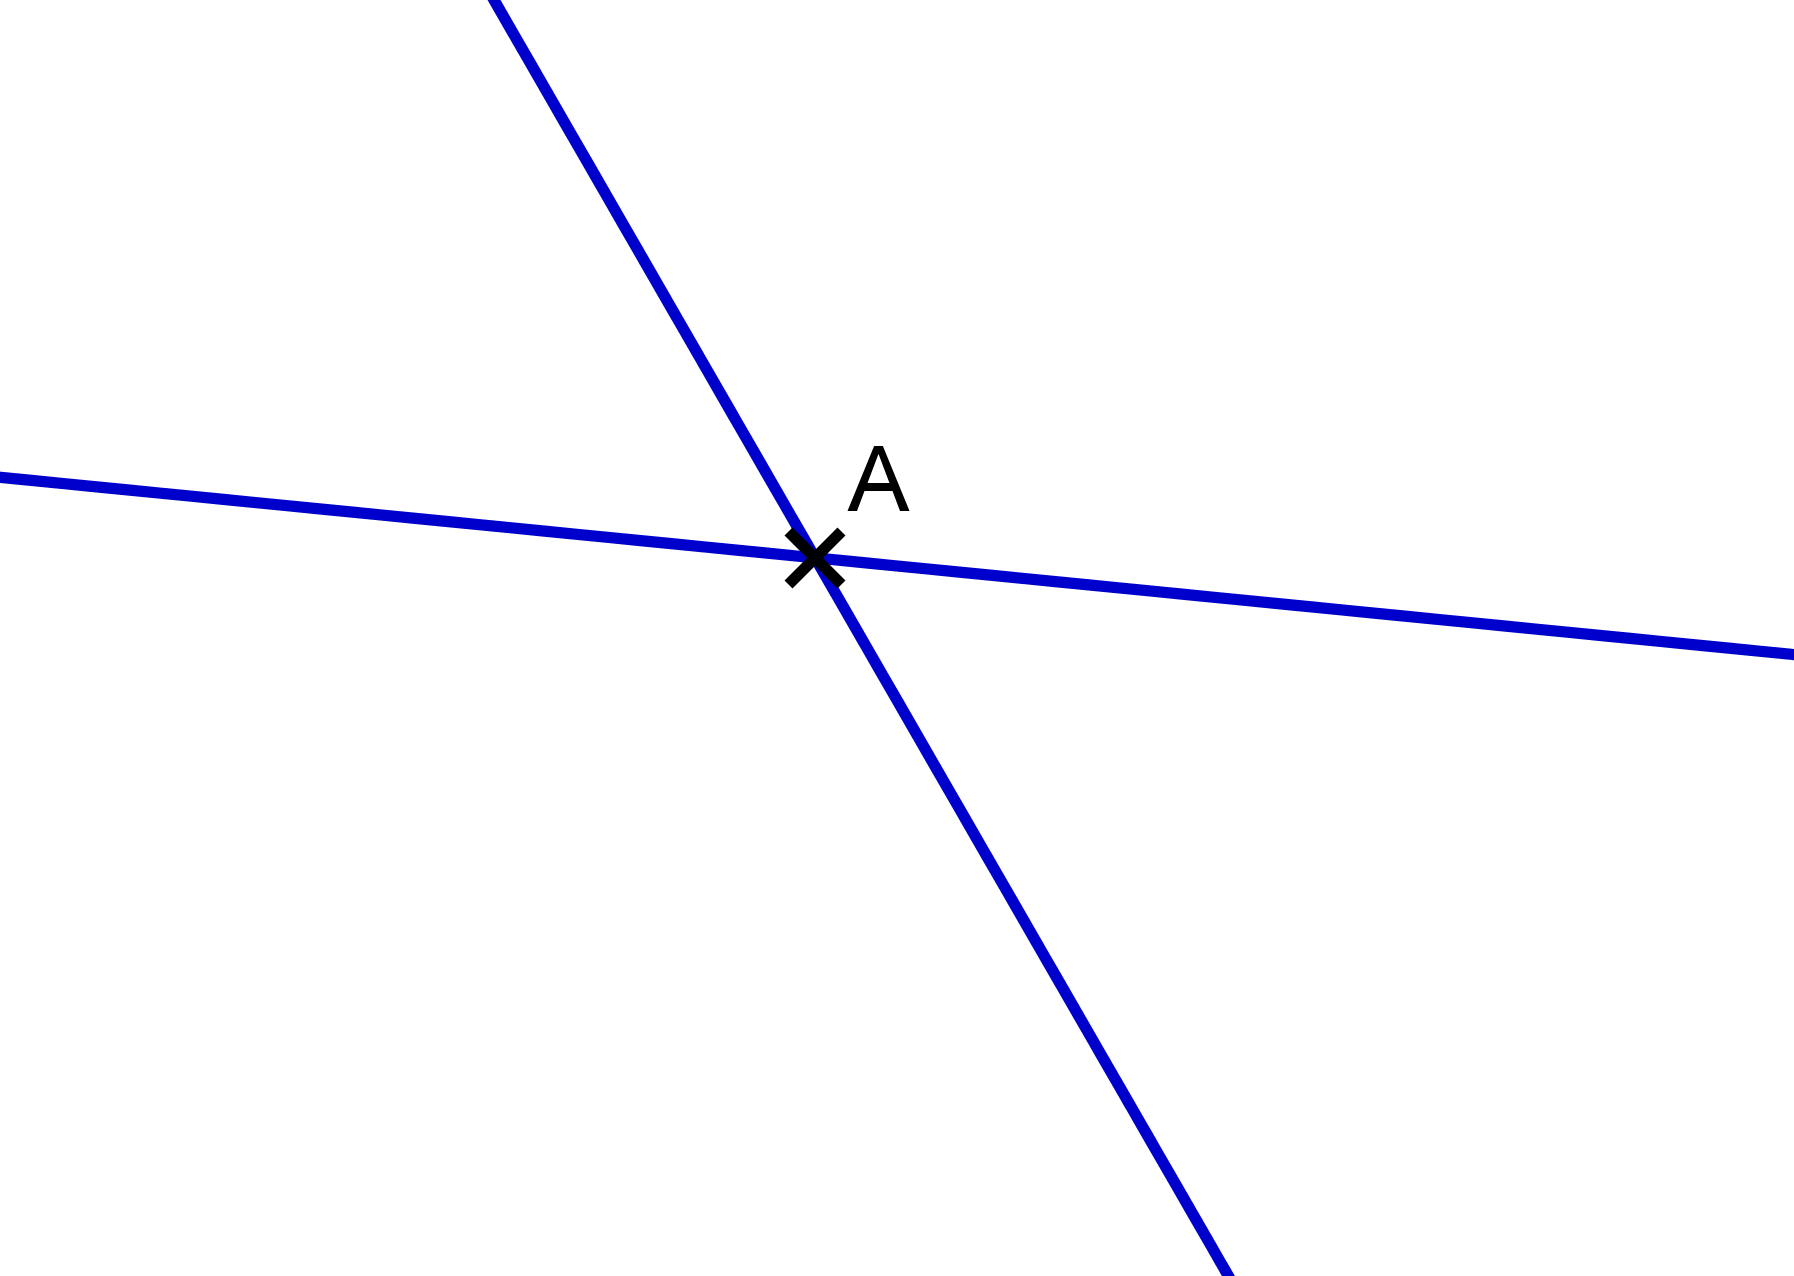
\includegraphics[width=5cm]{images/intersection.png}
\end{center}

\end{minipage}
\end{tabular}



\bigskip


\ul{D�finition}: Deux droites \textbf{perpendiculaires} sont deux droites
s�cantes qui forment un angle droit.




\enskip



\begin{tabular}{cc}
\begin{minipage}{12cm}



Les droites ($d_3$) et ($d_4$) sont perpendiculaires.


On note: $(d_3) \perp (d_4)$





 
\end{minipage}
&  
\begin{minipage}{6cm}

\begin{center}
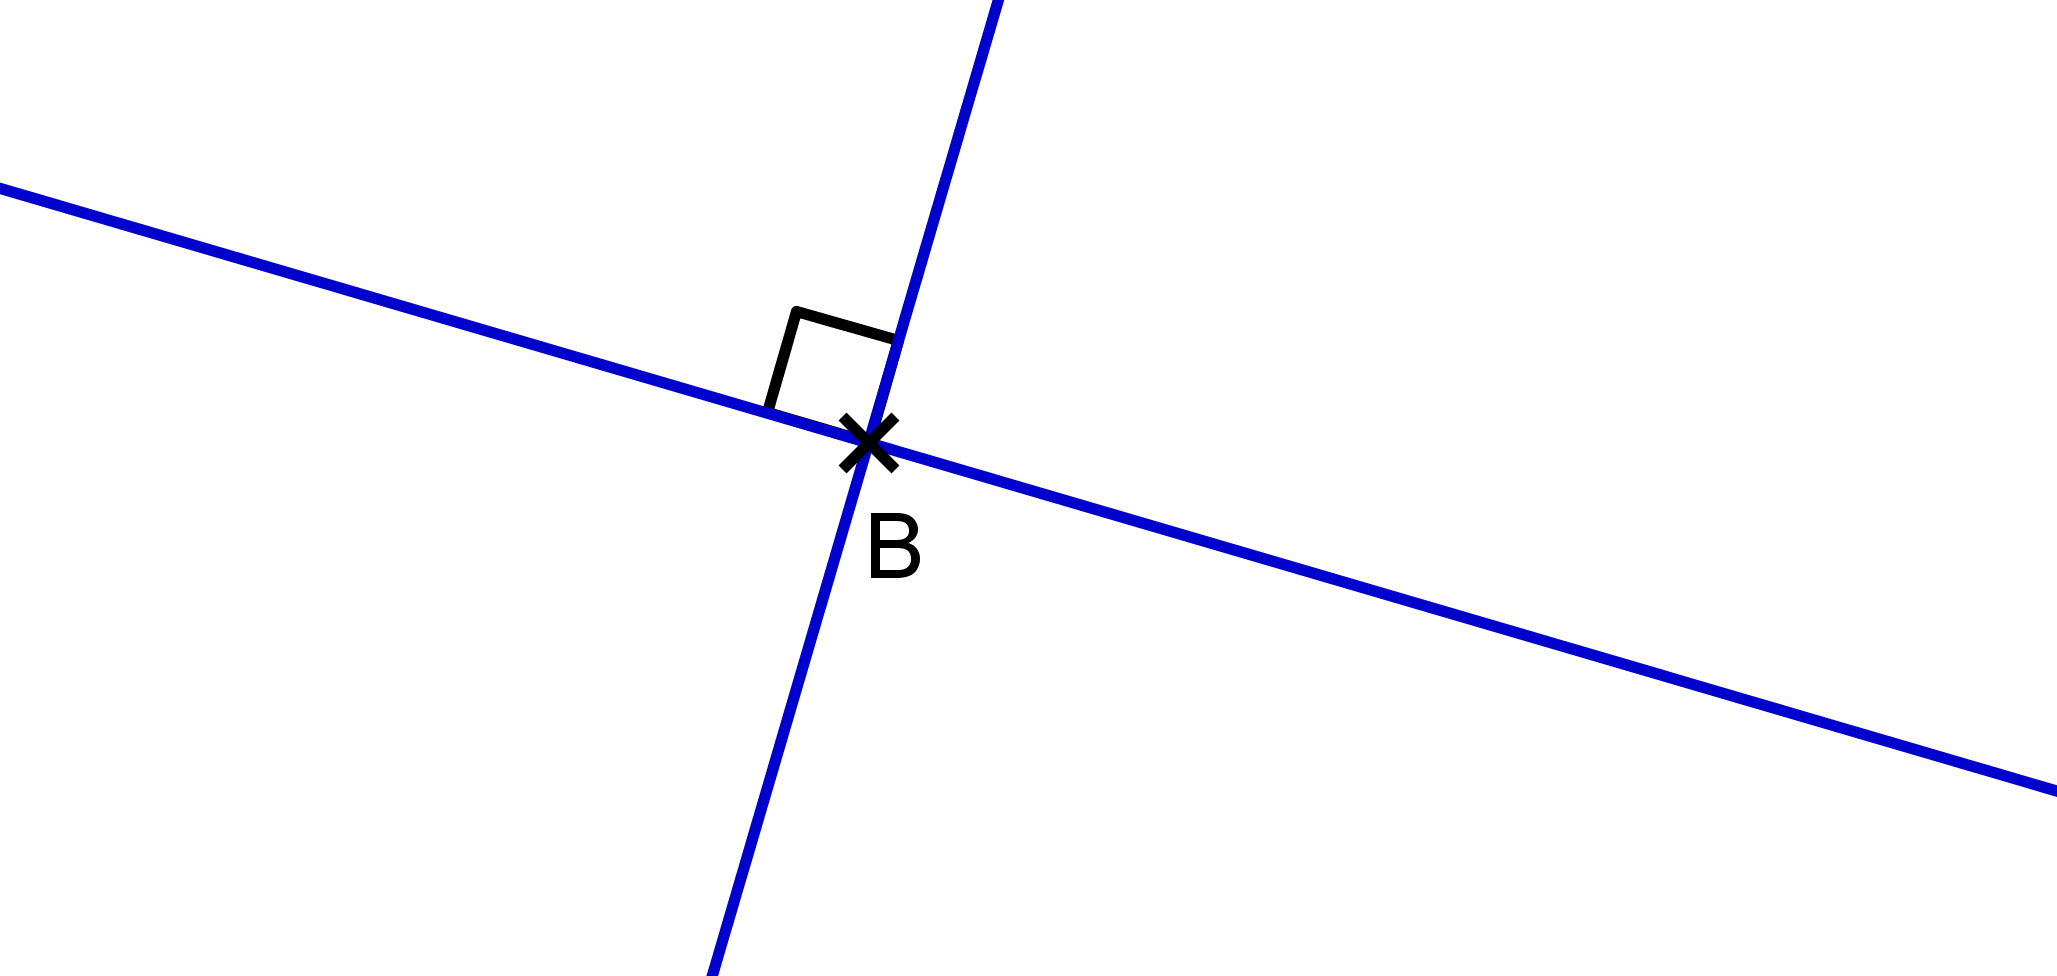
\includegraphics[width=5cm]{images/perpendiculaire.png}
\end{center}

\end{minipage}
\end{tabular}




\bigskip


\ul{D�finition}: Deux droites \textbf{parall�les} sont deux droites qui ne sont
pas s�cantes.

\enskip

\ul{Exemples}:
Les deux droites n'ont aucun point commun.



\begin{center}
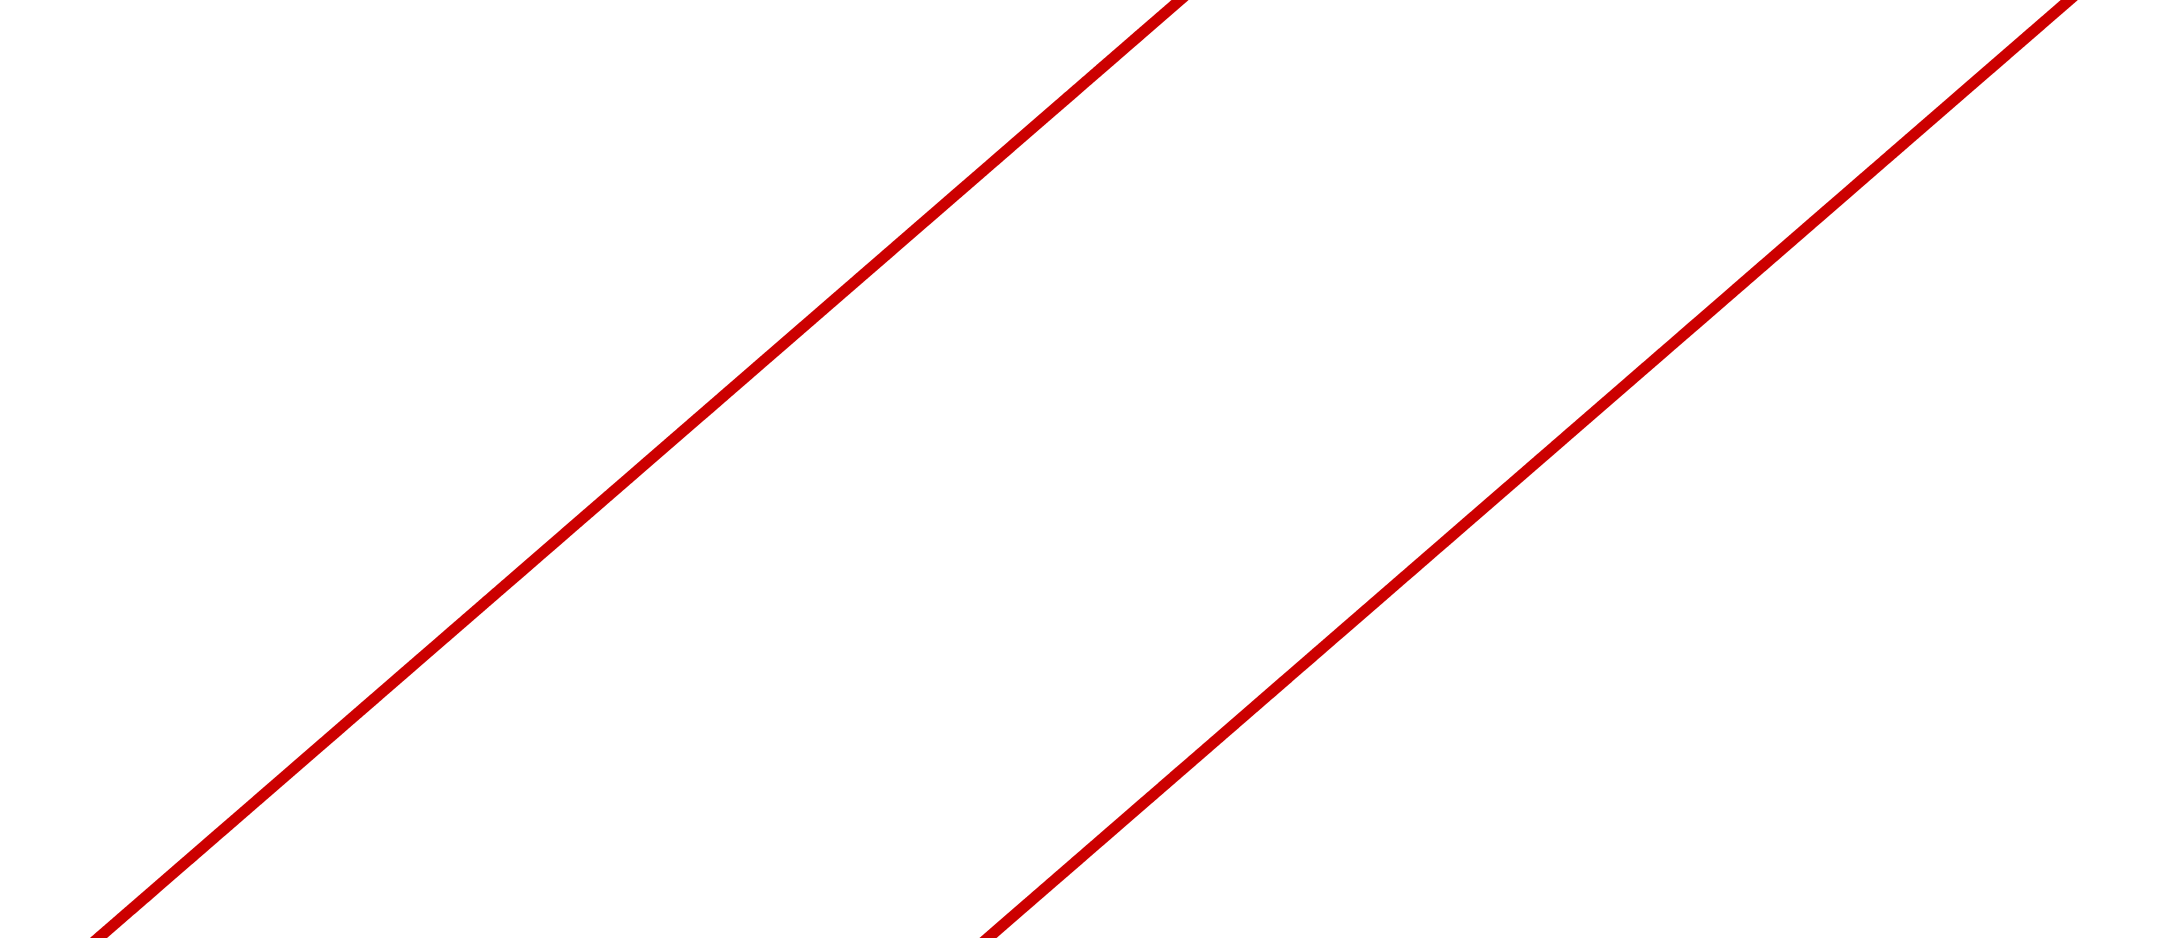
\includegraphics[width=4cm]{images/cas1.png}
\end{center}


Les droites ($d_1$) et ($d_2$) sont parall�les. 

On note: ($d_1$) // ($d_2$).





\subsection{Construction}




\ul{M�thode pour tracer des droites perpendiculaires}:
Tracer la droite (d') perpendiculaire � la droite (d) et passant par
le point A.

\begin{center}
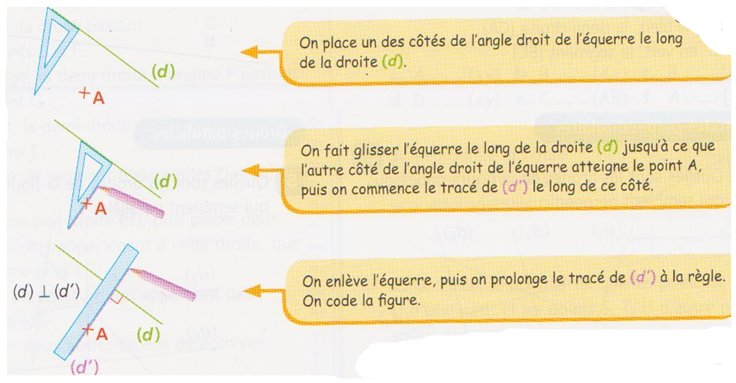
\includegraphics[width=15cm]{images/methode1.jpg}    
\end{center}



\bigskip



\ul{M�thode pour tracer des droites parall�les}:
Tracer la droite (d') perpendiculaire � la droite (d) et passant par
le point B.
 
\begin{center}
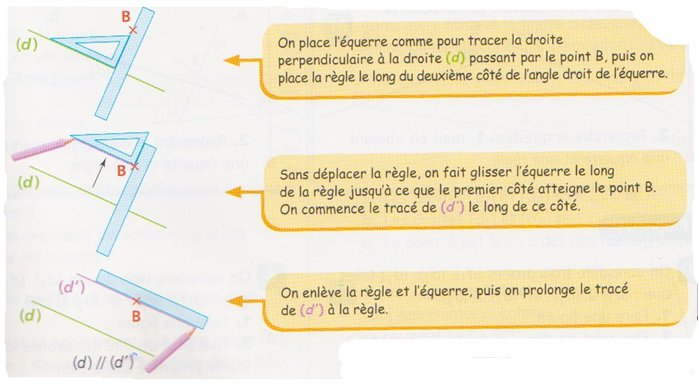
\includegraphics[width=15cm]{images/methode2.jpg}    
\end{center}
\end{document}
